
\section{Theorie}
\label{sec:Theorie}
Wenn Gamma-Strahlung Materie durchdringt wird ein Teil der Strahlung materialabhängig absorbiert und die abgeschwächte Intensität kann gemessen werden. Aus verschiedenen Messungen einer Schicht, die aus unterschiedlichen Richtungen erfolgen, entstehen bei einer Tomographie Projektionen, die schlussendlich zu einem 2D-Bild zusammen gesetzt werden können. Unter einer Projektion versteht man die Durchstrahlung eines Körpers mit einer bestimmten Ausrichtung. \\
\subsection{Wechselwirkung von Strahlung mit Materie}
In diesem Versuch wird ${}^{137}\mathrm{Cs}$ als Strahlungsquelle verwendet. Dies zerfällt zu 94,8\% in ${}^{137}\mathrm{Ba}$. Dies ist danach im angeregten Zustand. Um in den Grundzustand zu gelangen, entsendet es ein Photon mit der Energie von $\SI{661,7}{\kilo\electronvolt}$. In Abbildung (\ref{fig:caes}) ist dies dargestellt.
\begin{figure}
	\centering
	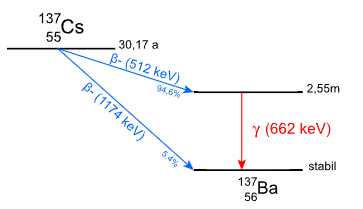
\includegraphics[scale=0.7]{fig/caes.png}
	\caption{Zerfall von ${}^{137}\mathrm{Cs}$ \cite{leifi}.}
	\label{fig:caes}
\end{figure}
\FloatBarrier
\noindent Die Absorption der Photonen erfolgt durch drei unterschiedlichen Effekte. Diese sind der Photo-Effekt, der Compton-Effekt und die Paarbildung, wobei alle drei auf der Wechselwirkung von Photonen mit Materie basieren.
Falls die Energie des Photons größer ist, als die des Hüllenelektron, wird das Elektron aus der Schale gelöst. Dies wird Photo-Effekt gennant, dafür muss gelten, dass $E_\gamma>E_\mathrm{Bindung}$.
Der Compton-Effekt ist eine inelastische Streuung vom Photon am Elektron. Dabei wird nur ein geringer Teil der Energie abgegeben. Bei der Paarbildung zerfällt das Photon unter Einfluss des Coulomb-Feldes des Atomkerns in ein Elektron und ein Positron. Dabei muss die Energie des Photons aufgrund der Energieerhaltung mindestens $E=\SI{1,02}{\mega\electronvolt}$ betragen.
Die drei Fälle unterscheiden sich in ihrer Häufigkeit im Verhältnis zur Energie.
Während der Photo-Effekt bei Energien bis $\SI{100}{\kilo\electronvolt}$ dominiert, tritt der Compton-Effekt von $\SI{100}{\kilo\electronvolt}$ bis $\SI{1}{\mega\electronvolt}$ auf. Die Paarbildung ist der stärkste Effekt ab einer Energie $E=\SI{1}{\mega\electronvolt}$.
Die Intensität nach dem Durchqueren des Materials kann über das Absorptionsgesetzt beschrieben werden, als:
\begin{align}
  \label{eqn:Ab}
  I=I_\mathrm{0} \exp\left(\sum_i \mu_\mathrm{i} d_\mathrm{i}\right)
\end{align}
Dabei ist $I$ die gemessene Intensität nach Durchquerung von Materie, $I_\mathrm{0}$ die Anfangsintensität, $\mu_\mathrm{i}$ der Absorptionskoeffizient, sowie $d_\mathrm{i}$ die Dicke des i-ten Materials.
Ein Spektrum der ${}^{137}\mathrm{Cs}$ Strahlung besteht im niedrigen Energiebereich aus einem Plateau aus Streuung, das nachfolgende Minimum ist die sogenannte Compton-Kante. Der darauffolgende Peak ist der Photo-Peak. In Abbildung (\ref{fig:spekt}) ist das Gammaspektrum von ${}^{137}\mathrm{Cs}$ dargestellt.
\begin{figure}
	\centering
	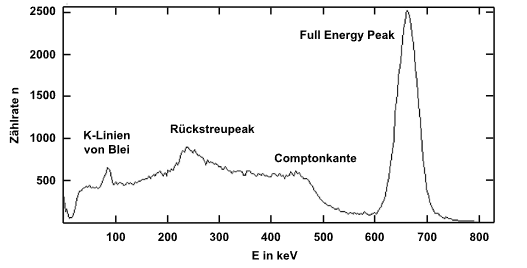
\includegraphics[scale=0.7]{fig/spek_cs.png}
	\caption{Gammaspektrum von ${}^{137}\mathrm{Cs}$ \cite{leifi}.}
	\label{fig:spekt}
\end{figure}
\FloatBarrier
\subsection{Bestimmung der Absorptionskoefizienten}
\noindent Durch Umstellung der Gleichung (\ref{eqn:Ab}) folgt:
\begin{align}
  \label{eqn:umab}
  \sum\limits_{I}^{}\mu_\mathrm{u} d_\mathrm{i} = \ln\left(\dfrac{I_\mathrm{0}}{I}\right)
\end{align}
Durch Zusammenfassen aller Dicken $d_\mathrm{i}$ in eine Geometriematrix $A$, aller Absorptionskoeffizienten $\mu$ in einen Vektor $\vec{\mu}$ und dem Vektor $\vec{I}$, der alle Verhältnisse zwischen $I$ und $I_\mathrm{0}$ enthält, ergibt sich:
\begin{align}
  \label{egn:Matrixschreibweise}
  A \vec{\mu} = \vec{I}
\end{align}
Um das Gleichungssystem zu lösen und den Fehler so klein wie möglich zu halten, muss das Gleichungssystem einerseits überbestimmt sein, andererseits wird die Methode der kleinsten Quadrate genutzt. Daraus folgt:
\begin{align}
  \label{eqn:Quadrate}
  W A \vec{\mu} = W \vec{I}
\end{align}
Mit der Gewichtungsmatrix $W=V[I]^{-1}$ ergibt sich:
\begin{align}
  \label{eqn:letzte Gleichung}
  \vec{\mu}=\left(A^TWA\right)^{-1}\left(A^TW\vec{I}\right)
\end{align}
Die Unsicherheiten sind gegeben durch:
\begin{equation}
  V[\mu]=\left(A^TWA\right)^{-1}
  \label{eqn:mu}
\end{equation}
